\section{Pattern\-Search Class Reference}
\label{classPatternSearch}\index{PatternSearch@{PatternSearch}}
{\tt \#include $<$Pattern\-Search.h$>$}

Inheritance diagram for Pattern\-Search::\begin{figure}[H]
\begin{center}
\leavevmode
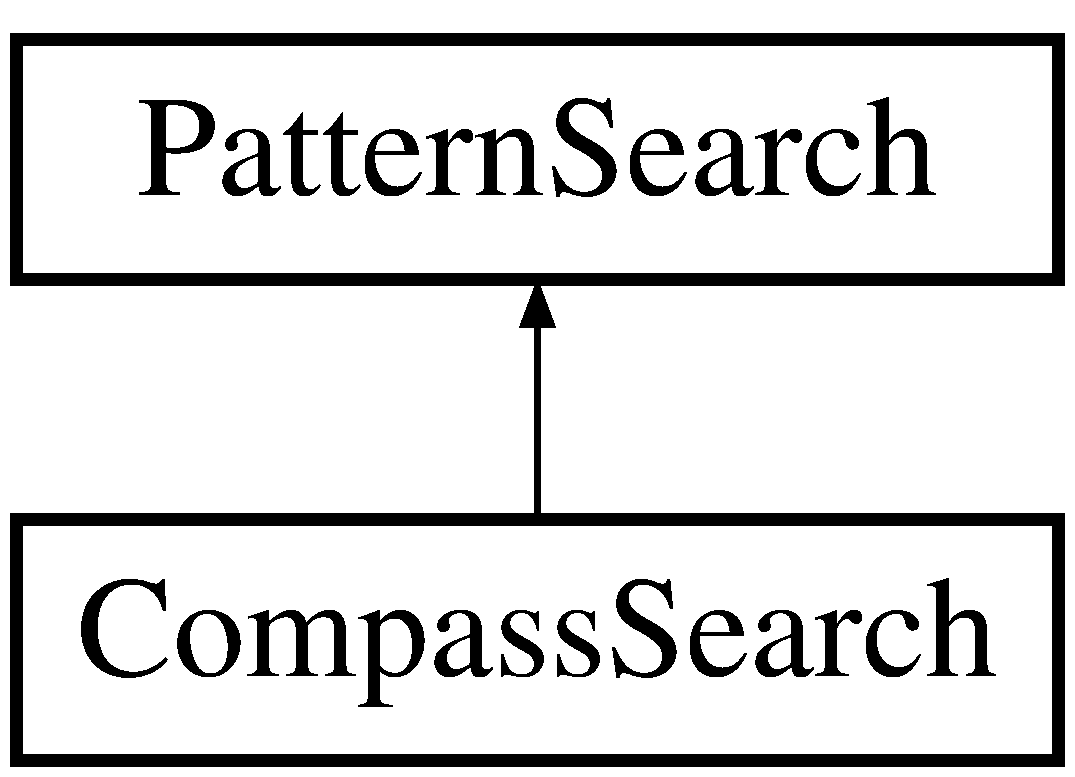
\includegraphics[height=2cm]{classPatternSearch}
\end{center}
\end{figure}
\subsection*{Public Member Functions}
\begin{Indent}{\bf Constructors \& Destructor}\par
\begin{CompactItemize}
\item 
{\bf Pattern\-Search} (long dim, Vector$<$ double $>$ \&start\-Point)
\item 
{\bf Pattern\-Search} (const {\bf Pattern\-Search} \&Original)
\item 
{\bf Pattern\-Search} (long dim, Vector$<$ double $>$ \&start\-Point, double start\-Step, double stop\-Step, void($\ast$objective)(long vars, Vector$<$ double $>$ \&x, double \&func, bool \&flag, void $\ast$an\_\-obj), void $\ast$input\_\-obj)
\item 
virtual {\bf $\sim$Pattern\-Search} ()
\end{CompactItemize}
\end{Indent}
\begin{Indent}{\bf Other Initialization Methods}\par
\begin{CompactItemize}
\item 
virtual {\bf Pattern\-Search} \& {\bf operator=} (const {\bf Pattern\-Search} \&A)
\item 
virtual void {\bf Clean\-Slate} (long dim, Vector$<$ double $>$ \&startpoint)
\item 
virtual void {\bf Clean\-Slate} (long dim, Vector$<$ double $>$ \&startpoint, double start\-Step, double stop\-Step, void($\ast$objective)(long vars, Vector$<$ double $>$ \&x, double \&func, bool \&flag, void $\ast$an\_\-obj), void $\ast$input\_\-obj)
\item 
void {\bf Initialize\-Design} (long pattern\-Size, const Matrix$<$ double $>$ $\ast$design\-Ptr)
\item 
void {\bf Read\-In\-File} (istream \&fp)
\item 
void {\bf Print\-Design} () const 
\end{CompactItemize}
\end{Indent}
\begin{Indent}{\bf Search method}\par
\begin{CompactItemize}
\item 
virtual void {\bf Begin\-Search} ()=0
\end{CompactItemize}
\end{Indent}
\begin{Indent}{\bf Accessors}\par
\begin{CompactItemize}
\item 
void {\bf Get\-Pattern\-Length} (long \&pattern) const 
\item 
double {\bf Get\-Delta} () const 
\item 
void {\bf Get\-Initial\-Step\-Length} (double \&step\-Len)
\item 
void {\bf Set\-Initial\-Step\-Length} (double \&step\-Len)
\end{CompactItemize}
\end{Indent}
\subsection*{Protected Member Functions}
\begin{CompactItemize}
\item 
virtual bool {\bf Stop} ()
\item 
virtual void {\bf Exploratory\-Moves} ()=0
\item 
virtual void {\bf Copy\-Search} (const {\bf Pattern\-Search} \&Original)
\item 
virtual void {\bf Next\-Point} (long index, const Vector$<$ double $>$ \&current\-Point, Vector$<$ double $>$ \&next\-Point)
\item 
virtual void {\bf Replace\-Minimum} (Vector$<$ double $>$ \&new\-Point, double new\-Value)
\item 
virtual void {\bf Scale\-Pattern} (double scalar)
\end{CompactItemize}
\subsection*{Protected Attributes}
\begin{CompactItemize}
\item 
long {\bf pattern\-Length}
\item 
double {\bf delta}
\item 
double {\bf initial\-Step\-Length}
\end{CompactItemize}


\subsection{Detailed Description}
The Pattern\-Search class is derived from the Direct\-Search class. Pattern\-Search is an abstract base class. 



\subsection{Constructor \& Destructor Documentation}
\index{PatternSearch@{Pattern\-Search}!PatternSearch@{PatternSearch}}
\index{PatternSearch@{PatternSearch}!PatternSearch@{Pattern\-Search}}
\subsubsection{\setlength{\rightskip}{0pt plus 5cm}Pattern\-Search::Pattern\-Search (long {\em dim}, Vector$<$ double $>$ \& {\em start\-Point})}\label{classPatternSearch_z15_0}


Constructor for class Pattern\-Search. This constructor has two parameters. Other data members will be set to default values, as follows (in addition to data members set by the Direct\-Search constructor): \{itemize\} [] pattern\-Length = 0 [] initial\-Step\-Length = .25 [] delta = initial\-Step\-Length [] IDnumber = 2000 \{itemize\}

\begin{Desc}
\item[Parameters:]
\begin{description}
\item[{\em dim}]the dimension of the problem \item[{\em startpoint}]the start point for the search \end{description}
\end{Desc}
\begin{Desc}
\item[See also:]Direct\-Search::Direct\-Search(long dim, Vector$<$double$>$ \&start\-Point) \end{Desc}
\index{PatternSearch@{Pattern\-Search}!PatternSearch@{PatternSearch}}
\index{PatternSearch@{PatternSearch}!PatternSearch@{Pattern\-Search}}
\subsubsection{\setlength{\rightskip}{0pt plus 5cm}Pattern\-Search::Pattern\-Search (const {\bf Pattern\-Search} \& {\em Original})}\label{classPatternSearch_z15_1}


Deep copy constructor for class Pattern\-Search \begin{Desc}
\item[Parameters:]
\begin{description}
\item[{\em Original}]a reference to the object to be copied. Note that this will in ordinary practice actually be a member of a concrete class derived from Pattern\-Search. \end{description}
\end{Desc}
\index{PatternSearch@{Pattern\-Search}!PatternSearch@{PatternSearch}}
\index{PatternSearch@{PatternSearch}!PatternSearch@{Pattern\-Search}}
\subsubsection{\setlength{\rightskip}{0pt plus 5cm}Pattern\-Search::Pattern\-Search (long {\em dim}, Vector$<$ double $>$ \& {\em start\-Point}, double {\em start\-Step}, double {\em stop\-Step}, void($\ast$)(long vars, Vector$<$ double $>$ \&x, double \&func, bool \&flag, void $\ast$an\_\-obj) {\em objective}, void $\ast$ {\em input\_\-obj})}\label{classPatternSearch_z15_2}


Special constructor using void function and object pointers. The objective function can be sent in as the fifth parameter here; the last parameter is used for any other information that may be necessary; it is used in MAPS, for example, to send in an object from an outside class. Usually, though, the final parameter will simply be set to NULL. This constructor takes six input parameters. \begin{Desc}
\item[Parameters:]
\begin{description}
\item[{\em dim}]the dimension of the problem \item[{\em start\-Point}]a Vector of doubles, the starting point for the search \item[{\em start\-Step}]the beginning delta, or lattice step length \item[{\em stop\-Step}]the stopping step length for the search \item[{\em objective}]a pointer to the function to be minimized \item[{\em input\_\-obj}]used to send additional data as needed--will normally be set to NULL. \end{description}
\end{Desc}
\index{PatternSearch@{Pattern\-Search}!~PatternSearch@{$\sim$PatternSearch}}
\index{~PatternSearch@{$\sim$PatternSearch}!PatternSearch@{Pattern\-Search}}
\subsubsection{\setlength{\rightskip}{0pt plus 5cm}virtual Pattern\-Search::$\sim${\bf Pattern\-Search} ()\hspace{0.3cm}{\tt  [virtual]}}\label{classPatternSearch_z15_3}


Destructor 

\subsection{Member Function Documentation}
\index{PatternSearch@{Pattern\-Search}!BeginSearch@{BeginSearch}}
\index{BeginSearch@{BeginSearch}!PatternSearch@{Pattern\-Search}}
\subsubsection{\setlength{\rightskip}{0pt plus 5cm}virtual void Pattern\-Search::Begin\-Search ()\hspace{0.3cm}{\tt  [pure virtual]}}\label{classPatternSearch_z19_0}


\{ {\bf Begin\-Search()}{\rm (p.\,\pageref{classPatternSearch_z19_0})}\} is an unimplemented virtual void method in the abstract base classes. It is to be implemented in the concrete classes. There, {\bf Begin\-Search()}{\rm (p.\,\pageref{classPatternSearch_z19_0})} will call the methods that implement the actual search algorithms. 

Implemented in {\bf Compass\-Search} {\rm (p.\,\pageref{classCompassSearch_z5_1})}.\index{PatternSearch@{Pattern\-Search}!CleanSlate@{CleanSlate}}
\index{CleanSlate@{CleanSlate}!PatternSearch@{Pattern\-Search}}
\subsubsection{\setlength{\rightskip}{0pt plus 5cm}virtual void Pattern\-Search::Clean\-Slate (long {\em dim}, Vector$<$ double $>$ \& {\em startpoint}, double {\em start\-Step}, double {\em stop\-Step}, void($\ast$)(long vars, Vector$<$ double $>$ \&x, double \&func, bool \&flag, void $\ast$an\_\-obj) {\em objective}, void $\ast$ {\em input\_\-obj})\hspace{0.3cm}{\tt  [virtual]}}\label{classPatternSearch_z17_2}


overloaded version of \{ Clean\-Slate\} using void function and object pointers. This version of Clean\-Slate takes six parameters. \begin{Desc}
\item[Parameters:]
\begin{description}
\item[{\em dim}]the dimension of the problem \item[{\em start\-Point}]a Vector of doubles, the starting point for the search \item[{\em start\-Step}]the beginning delta, or lattice step length \item[{\em stop\-Step}]the stopping step length for the search \item[{\em objective}]a pointer to the function to be minimized \item[{\em input\_\-obj}]used to send additional data as needed--will normally be set to NULL. \end{description}
\end{Desc}
\begin{Desc}
\item[Returns:]void \end{Desc}
\begin{Desc}
\item[See also:]{\bf Clean\-Slate(long dim, Vector$<$double$>$ \&startpoint)}{\rm (p.\,\pageref{classPatternSearch_z17_1})} \end{Desc}
\index{PatternSearch@{Pattern\-Search}!CleanSlate@{CleanSlate}}
\index{CleanSlate@{CleanSlate}!PatternSearch@{Pattern\-Search}}
\subsubsection{\setlength{\rightskip}{0pt plus 5cm}virtual void Pattern\-Search::Clean\-Slate (long {\em dim}, Vector$<$ double $>$ \& {\em startpoint})\hspace{0.3cm}{\tt  [virtual]}}\label{classPatternSearch_z17_1}


Reinitializes values in order to reuse the same search object. This version of \{ Clean\-Slate\} takes two parameters. Other data members are set by default as in the constructor {\bf Pattern\-Search(long, Vector$<$double$>$\&)}{\rm (p.\,\pageref{classPatternSearch_z15_0})}. \begin{Desc}
\item[Parameters:]
\begin{description}
\item[{\em dim}]the dimension of the problem \item[{\em start\-Point}]the new starting point for the search \end{description}
\end{Desc}
\begin{Desc}
\item[Returns:]void \end{Desc}
\begin{Desc}
\item[See also:]{\bf Clean\-Slate}{\rm (p.\,\pageref{classPatternSearch_z17_1})}(long dim, Vector$<$double$>$ \&startpoint, double$\ast$ start\-Step, double stop\-Step, void ($\ast$objective)(long vars, Vector$<$double$>$ \&x, double \& func, bool\& flag, void$\ast$ an\_\-obj), void $\ast$ input\_\-obj) \end{Desc}
\index{PatternSearch@{Pattern\-Search}!CopySearch@{CopySearch}}
\index{CopySearch@{CopySearch}!PatternSearch@{Pattern\-Search}}
\subsubsection{\setlength{\rightskip}{0pt plus 5cm}virtual void Pattern\-Search::Copy\-Search (const {\bf Pattern\-Search} \& {\em Original})\hspace{0.3cm}{\tt  [protected, virtual]}}\label{classPatternSearch_b2}


Used to implement the overloaded assignment operator. \begin{Desc}
\item[Parameters:]
\begin{description}
\item[{\em Original}]a reference to a Pattern\-Search object \end{description}
\end{Desc}
\begin{Desc}
\item[Returns:]void \end{Desc}
\index{PatternSearch@{Pattern\-Search}!ExploratoryMoves@{ExploratoryMoves}}
\index{ExploratoryMoves@{ExploratoryMoves}!PatternSearch@{Pattern\-Search}}
\subsubsection{\setlength{\rightskip}{0pt plus 5cm}virtual void Pattern\-Search::Exploratory\-Moves ()\hspace{0.3cm}{\tt  [protected, pure virtual]}}\label{classPatternSearch_b1}


Pattern\-Search::Exploratory Moves is an unimplemented virtual void function. It will be implemented in the concrete classes as the workhorse for the algorithmic implementations 

Implemented in {\bf Compass\-Search} {\rm (p.\,\pageref{classCompassSearch_b0})}.\index{PatternSearch@{Pattern\-Search}!GetDelta@{GetDelta}}
\index{GetDelta@{GetDelta}!PatternSearch@{Pattern\-Search}}
\subsubsection{\setlength{\rightskip}{0pt plus 5cm}double Pattern\-Search::Get\-Delta () const}\label{classPatternSearch_z21_1}


Returns delta, the lattice step length \begin{Desc}
\item[Returns:]double \end{Desc}
\index{PatternSearch@{Pattern\-Search}!GetInitialStepLength@{GetInitialStepLength}}
\index{GetInitialStepLength@{GetInitialStepLength}!PatternSearch@{Pattern\-Search}}
\subsubsection{\setlength{\rightskip}{0pt plus 5cm}void Pattern\-Search::Get\-Initial\-Step\-Length (double \& {\em step\-Len})}\label{classPatternSearch_z21_2}


Returns initial\-Step\-Length, the initial value of delta. \begin{Desc}
\item[Parameters:]
\begin{description}
\item[{\em step\-Len}]a reference to a double: will be assigned the value of initial\-Step\-Length \end{description}
\end{Desc}
\begin{Desc}
\item[Returns:]void \end{Desc}
\index{PatternSearch@{Pattern\-Search}!GetPatternLength@{GetPatternLength}}
\index{GetPatternLength@{GetPatternLength}!PatternSearch@{Pattern\-Search}}
\subsubsection{\setlength{\rightskip}{0pt plus 5cm}void Pattern\-Search::Get\-Pattern\-Length (long \& {\em pattern}) const}\label{classPatternSearch_z21_0}


Returns the number of \char`\"{}columns\char`\"{} of the pattern matrix \begin{Desc}
\item[Parameters:]
\begin{description}
\item[{\em pattern}]a long provided by the user; will be assigned the value of pattern\-Length \end{description}
\end{Desc}
\begin{Desc}
\item[Returns:]void \end{Desc}
\index{PatternSearch@{Pattern\-Search}!InitializeDesign@{InitializeDesign}}
\index{InitializeDesign@{InitializeDesign}!PatternSearch@{Pattern\-Search}}
\subsubsection{\setlength{\rightskip}{0pt plus 5cm}void Pattern\-Search::Initialize\-Design (long {\em pattern\-Size}, const Matrix$<$ double $>$ $\ast$ {\em design\-Ptr})}\label{classPatternSearch_z17_3}


Deletes any existing pattern and replaces it with the one pointed to by design\-Ptr. Calls Design\-Search::Initialize\-Design() and then initializes pattern\-Length. \begin{Desc}
\item[Parameters:]
\begin{description}
\item[{\em pattern\-Size}]the number of \char`\"{}columns\char`\"{}, i.e. trial points, in design matrix \item[{\em pat}]a pointer to a design matrix \end{description}
\end{Desc}
\begin{Desc}
\item[Returns:]void \end{Desc}
\index{PatternSearch@{Pattern\-Search}!NextPoint@{NextPoint}}
\index{NextPoint@{NextPoint}!PatternSearch@{Pattern\-Search}}
\subsubsection{\setlength{\rightskip}{0pt plus 5cm}virtual void Pattern\-Search::Next\-Point (long {\em index}, const Vector$<$ double $>$ \& {\em current\-Point}, Vector$<$ double $>$ \& {\em next\-Point})\hspace{0.3cm}{\tt  [protected, virtual]}}\label{classPatternSearch_b3}


{\bf Next\-Point()}{\rm (p.\,\pageref{classPatternSearch_b3})} calculates the next trial point by adding the design matrix column at index to the current vector. Returns the prospect in next\-Point. \begin{Desc}
\item[Parameters:]
\begin{description}
\item[{\em index}]the index of a column of the design matrix \item[{\em current\-Point}]a reference to the current vector \item[{\em next\-Point}]a reference to a vector, which will be assigned the value of the appropriate point to be evaluated next. \end{description}
\end{Desc}
\begin{Desc}
\item[Returns:]void \end{Desc}
\index{PatternSearch@{Pattern\-Search}!operator=@{operator=}}
\index{operator=@{operator=}!PatternSearch@{Pattern\-Search}}
\subsubsection{\setlength{\rightskip}{0pt plus 5cm}virtual {\bf Pattern\-Search}\& Pattern\-Search::operator= (const {\bf Pattern\-Search} \& {\em A})\hspace{0.3cm}{\tt  [virtual]}}\label{classPatternSearch_z17_0}


Overloaded assignment operator. note that because Pattern\-Search is an abstract base class, the object actually returned will be of a type corresponding to one of the concrete classes. \begin{Desc}
\item[Parameters:]
\begin{description}
\item[{\em A}]reference to a const Pattern\-Search object \end{description}
\end{Desc}
\begin{Desc}
\item[Returns:]Pattern\-Search\& \end{Desc}
\index{PatternSearch@{Pattern\-Search}!PrintDesign@{PrintDesign}}
\index{PrintDesign@{PrintDesign}!PatternSearch@{Pattern\-Search}}
\subsubsection{\setlength{\rightskip}{0pt plus 5cm}void Pattern\-Search::Print\-Design () const}\label{classPatternSearch_z17_5}


Prints out useful information about the search \index{PatternSearch@{Pattern\-Search}!ReadInFile@{ReadInFile}}
\index{ReadInFile@{ReadInFile}!PatternSearch@{Pattern\-Search}}
\subsubsection{\setlength{\rightskip}{0pt plus 5cm}void Pattern\-Search::Read\-In\-File (istream \& {\em fp})}\label{classPatternSearch_z17_4}


Reads the design in from a file. You may also pass cin as the input stream as desired. Input first the pattern length and then the values of each trial vector (i.e. input the pattern by column) \begin{Desc}
\item[Parameters:]
\begin{description}
\item[{\em fp}]the filestream --or cin may be used \end{description}
\end{Desc}
\begin{Desc}
\item[Returns:]void \end{Desc}
\index{PatternSearch@{Pattern\-Search}!ReplaceMinimum@{ReplaceMinimum}}
\index{ReplaceMinimum@{ReplaceMinimum}!PatternSearch@{Pattern\-Search}}
\subsubsection{\setlength{\rightskip}{0pt plus 5cm}virtual void Pattern\-Search::Replace\-Minimum (Vector$<$ double $>$ \& {\em new\-Point}, double {\em new\-Value})\hspace{0.3cm}{\tt  [protected, virtual]}}\label{classPatternSearch_b4}


Replaces the minimizer \& the minimum objective function value. \begin{Desc}
\item[Parameters:]
\begin{description}
\item[{\em new\-Point}]the point that will be assigned as the new min\-Point \item[{\em new\-Value}]the value that will be assigned to min\-Value \end{description}
\end{Desc}
\begin{Desc}
\item[Returns:]void \end{Desc}
\index{PatternSearch@{Pattern\-Search}!ScalePattern@{ScalePattern}}
\index{ScalePattern@{ScalePattern}!PatternSearch@{Pattern\-Search}}
\subsubsection{\setlength{\rightskip}{0pt plus 5cm}virtual void Pattern\-Search::Scale\-Pattern (double {\em scalar})\hspace{0.3cm}{\tt  [protected, virtual]}}\label{classPatternSearch_b5}


Scale lattice step length by scalar \begin{Desc}
\item[Parameters:]
\begin{description}
\item[{\em scalar}]the value by which to scale the pattern \end{description}
\end{Desc}
\begin{Desc}
\item[Returns:]void \end{Desc}
\index{PatternSearch@{Pattern\-Search}!SetInitialStepLength@{SetInitialStepLength}}
\index{SetInitialStepLength@{SetInitialStepLength}!PatternSearch@{Pattern\-Search}}
\subsubsection{\setlength{\rightskip}{0pt plus 5cm}void Pattern\-Search::Set\-Initial\-Step\-Length (double \& {\em step\-Len})}\label{classPatternSearch_z21_3}


Assigns the value of steplen to initial\-Step\-Length. \begin{Desc}
\item[Parameters:]
\begin{description}
\item[{\em step\-Len}]a reference to a double:initial\-Step\-Length will be assigned this value. \end{description}
\end{Desc}
\begin{Desc}
\item[Returns:]void \end{Desc}
\index{PatternSearch@{Pattern\-Search}!Stop@{Stop}}
\index{Stop@{Stop}!PatternSearch@{Pattern\-Search}}
\subsubsection{\setlength{\rightskip}{0pt plus 5cm}virtual bool Pattern\-Search::Stop ()\hspace{0.3cm}{\tt  [protected, virtual]}}\label{classPatternSearch_b0}


Whether nor not to stop, based either on max\-Calls or lattice resolution \begin{Desc}
\item[Returns:]bool \end{Desc}


\subsection{Member Data Documentation}
\index{PatternSearch@{Pattern\-Search}!delta@{delta}}
\index{delta@{delta}!PatternSearch@{Pattern\-Search}}
\subsubsection{\setlength{\rightskip}{0pt plus 5cm}double {\bf Pattern\-Search::delta}\hspace{0.3cm}{\tt  [protected]}}\label{classPatternSearch_p1}


The density of the underlying lattice \index{PatternSearch@{Pattern\-Search}!initialStepLength@{initialStepLength}}
\index{initialStepLength@{initialStepLength}!PatternSearch@{Pattern\-Search}}
\subsubsection{\setlength{\rightskip}{0pt plus 5cm}double {\bf Pattern\-Search::initial\-Step\-Length}\hspace{0.3cm}{\tt  [protected]}}\label{classPatternSearch_p2}


The initial setting for delta \index{PatternSearch@{Pattern\-Search}!patternLength@{patternLength}}
\index{patternLength@{patternLength}!PatternSearch@{Pattern\-Search}}
\subsubsection{\setlength{\rightskip}{0pt plus 5cm}long {\bf Pattern\-Search::pattern\-Length}\hspace{0.3cm}{\tt  [protected]}}\label{classPatternSearch_p0}


The number of \char`\"{}columns\char`\"{} in design matrix, i.e. trial points 

The documentation for this class was generated from the following file:\begin{CompactItemize}
\item 
Pattern\-Search.h\end{CompactItemize}
